\documentclass[12pt]{article}

\usepackage{sbc-template}
\usepackage{cite}
\usepackage{graphicx,url}
\usepackage[utf8]{inputenc}
\usepackage[brazil]{babel} 

     
\sloppy

\title{Aplicação de \textit{Automatic Number Plate Recognition} (ANPR) no controle de acesso de veículos}

\author{Maurício de A. Cordeiro\inst{1} }

\address{Instituto Federal de Educação, Ciência e Tecnologia da Bahia\\ 
	Avenida Sérgio Vieira Melo, 3150. Bairro Zabelê - Vitória da Conquista - BA - Brasil\\
	CEP 45078-900
  \email{mauriciocordeiro@live.com}
}

\begin{document} 

\maketitle

\begin{abstract}
  \textit{soon...}
\end{abstract}
     
\begin{resumo} 
 Este trabalho consiste no desenvolvimento de sistema para controle de acesso de veículos baseado em ANPR (\textit{Automatic Number Plate Recognition}), com largo potencial de sua aplicação em locais ou espaços físicos que exigem algum nível de segurança, quando da entrada e saída de pessoas (a título de exemplo, citam-se aqui condomínios e estacionamentos privados). 
\end{resumo}

\section{Introdução}

Lorem ipsum dolor sit amet, consectetur adipiscing elit. Vivamus tristique augue in diam accumsan, ac pellentesque tortor rutrum. Maecenas sollicitudin lorem nec turpis egestas consequat. Ut ornare, lorem sed aliquam tincidunt, massa erat luctus nulla, id malesuada velit risus quis leo. Nulla facilisi. Maecenas non sodales lectus, eu lacinia nibh. Vestibulum tortor ligula, pellentesque sed vestibulum quis, suscipit nec augue. Ut ac augue non ex dictum laoreet ut sed diam. Vestibulum pretium tellus quis nisl iaculis, interdum viverra felis fermentum. Aenean rhoncus vitae neque id tempor. Nulla ac turpis cursus, fermentum ante et, dignissim dui. Suspendisse et odio dapibus, lacinia justo vel, fermentum nibh. Nam a ligula in nisi pretium aliquam. Aenean volutpat justo est, et dignissim tellus tempor non. Praesent imperdiet erat non quam efficitur, a tincidunt diam mollis. Nam convallis lacus nec nisl dignissim efficitur.

Quisque cursus quis odio a tincidunt. Maecenas vel purus sagittis, suscipit lectus a, pellentesque magna. Morbi sagittis, quam quis suscipit suscipit, lectus justo egestas felis, sed vehicula elit lorem vitae ante. Nam lacinia interdum ullamcorper. Nulla lorem est, placerat id convallis id, consequat eu lorem. Aliquam est enim, viverra ac lacinia in, lacinia at risus. Mauris maximus urna ornare enim interdum ornare a id metus. Sed non aliquet diam, sed tristique erat. Vestibulum congue mi et ligula faucibus malesuada.

Donec ornare venenatis magna. Aenean facilisis tincidunt vestibulum. Quisque at lorem vitae mauris sollicitudin sodales interdum et diam. Suspendisse potenti. Vestibulum eget rutrum tortor. Nulla vel scelerisque justo, tincidunt consectetur mauris. Cras vulputate rhoncus justo, facilisis elementum magna pretium et. Curabitur mollis massa risus, non efficitur neque ullamcorper in. Etiam imperdiet pellentesque tortor et efficitur. Fusce sed nisi in turpis cursus vehicula. Nulla pellentesque, purus vitae interdum sodales, mauris ipsum fermentum sem, ac vestibulum augue lorem in nulla. Donec quis ligula nibh. Fusce pretium mauris quis turpis convallis mollis. 

\subsection{Trabalhos correlatos}

Lorem ipsum dolor sit amet, consectetur adipiscing elit. Vivamus tristique augue in diam accumsan, ac pellentesque tortor rutrum. Maecenas sollicitudin lorem nec turpis egestas consequat. Ut ornare, lorem sed aliquam tincidunt, massa erat luctus nulla, id malesuada velit risus quis leo. Nulla facilisi. Maecenas non sodales lectus, eu lacinia nibh. Vestibulum tortor ligula, pellentesque sed vestibulum quis, suscipit nec augue. Ut ac augue non ex dictum laoreet ut sed diam. Vestibulum pretium tellus quis nisl iaculis, interdum viverra felis fermentum. Aenean rhoncus vitae neque id tempor. Nulla ac turpis cursus, fermentum ante et, dignissim dui. Suspendisse et odio dapibus, lacinia justo vel, fermentum nibh. Nam a ligula in nisi pretium aliquam. Aenean volutpat justo est, et dignissim tellus tempor non. Praesent imperdiet erat non quam efficitur, a tincidunt diam mollis. Nam convallis lacus nec nisl dignissim efficitur. 


\section{Arquitetura} \label{sec:architecture}

A solução desenvolvida neste trabalho é baseia-se na arquitetura de microsserviços, com módulos virtuais conteinerizados, que se comunicam via HTTP, além da aplicação de tecnologias baseadas em ANPR. Esta seção se dedica a detalhar esses conceitos.

\subsection{Arquitetura de Microsserviços}

Arquitetura de Microsserviços (\textit{Microservices Architecture} - MSA) é um modelo arquitetural onde processos de \textit{software} são realizados por componentes fracamente acoplados, que possuem funcionalidades específicas e bem definidas, e que se comunicam através de interfaces padronizadas \cite{viggiato2018}.

A MSA pode ser considerada como a segunda iteração da Arquitetura Orientada a Serviços (\textit{Service Oriented Architecture} - SOA), onde serviços complexos são decompostos em partes mais flexíveis, especializadas e de fácil manutenção, de modo que cada uma é responsável por uma única e pequena funcionalidade com o intuito de realizá-la bem \cite{homay2019}. 

\subsection{Virtualização baseada em contêiner}

A Virtualização baseada em contêiner \cite{eder2016} consiste na utilização de recursos de \textit{hardware} e do \textit{kernel} de um sistema hospedeiro a fim de criar ambientes isolados para a execução de determinados processos, o chamado \textbf{contêiner}, esquematizado na Figura~\ref{fig:conteiner}.

\begin{figure}[ht]
	\centering
	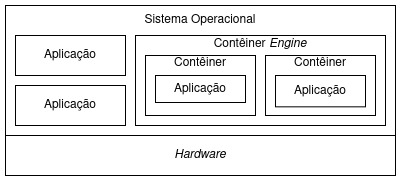
\includegraphics[width=.8\textwidth]{conteiner.jpg}
	\caption{Virtualização baseada em contêiner}
	\label{fig:conteiner}
\end{figure} 

Nessa abordagem, o contêiner aloca apenas os recursos necessário para executar sua aplicação, enquanto trabalha isolado de outros contêineres que possam estar em execução em um mesmo hospedeiro. Essa característica corrobora com sua utilidade quanto a aplicação em soluções baseadas de MSA, uma vez que os contêineres são capazes de se comunicar entre si.

\subsection{REST}

O REST (\textit{REpresentational State Transfer}) é uma implementação da SOA sobre o HTTP para transferência de representações de um determinado recurso entre cliente e servidor \cite{mumbaikar2013}.

De forma geral, o REST estabelece semântica para métodos e URI (\textit{Universal Resource Identifier}) no HTTP, padronizando a forma como recursos são solicitados e disponibilizados na web (Figura~\ref{fig:rest}). Nesse contexto, leia-se "recurso" como um item acessível via URI e a "semântica do método" padroniza o modo de interação com o recurso, como, por exemplo, \texttt{POST} para criar, \texttt{GET} para solicitar, \texttt{PUT} para editar e \texttt{DELETE} para remover \cite{adamczyk2011}.

\begin{figure}[ht]
	\centering
	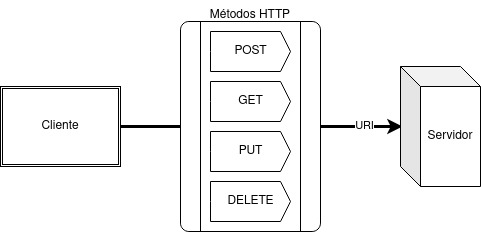
\includegraphics[width=.8\textwidth]{rest.jpg}
	\caption{Comunicação cliente-servidor com REST}
	\label{fig:rest}
\end{figure} 

\subsection{ANPR}

O ANPR (\textit{Automatic Number Plate Recognition}), que possui papel central na solução desenvolvida neste trabalho, é uma tecnologia que utiliza de visão computacional e processamento de imagem para identificar e reconhecer caracteres em placas de veículos.

Existem diferentes técnicas e algoritmos que podem seu usados no ANPR, mas, de forma geral, todos eles seguem um processo com etapas bem definidas \cite{mufti2021}: (i) Extração da placa, (ii) Segmentação de caracteres e (iii) Reconhecimento de caracteres.

Dentro das etapas para a execução do ANPR, \cite{shashirangana2020} pode-se classificar as diferentes técnicas (que vão desde algoritmos de processamento de imagens até aplicação de redes neurais para classificação de objetos) conforme o mostrado na Figura~\ref{fig:anpr-steps}:

\begin{figure}[ht]
	\centering
	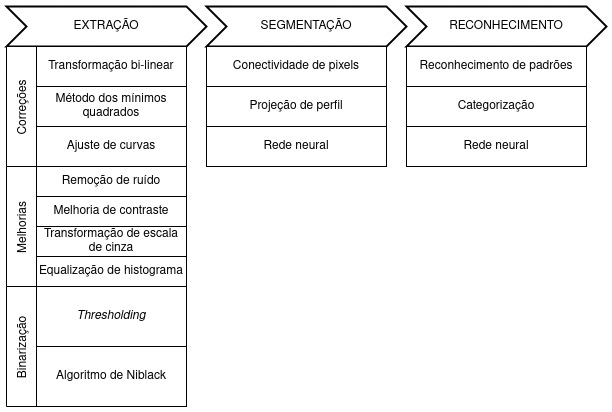
\includegraphics[width=.8\textwidth]{anpr-steps.jpg}
	\caption{Etapas e técnicas aplicadas no ANPR}
	\label{fig:anpr-steps}
\end{figure} 


\section{Sistema para controle de acesso de veículos baseado em ANPR}

O sistema para controle de acesso de veículos implementado neste trabalho foi organizado em módulos, ou contêineres, cada um com uma funcionalidade específica (seguindo os princípios da MSA), que se comunicam direta ou indiretamente entre si, como mostrado na Figura~\ref{fig:anpr-auth}. Esses módulos foram implementados com ferramentas tais como: Docker, Java, Python, Angular e MongoDB.

\begin{figure}[ht]
	\centering
	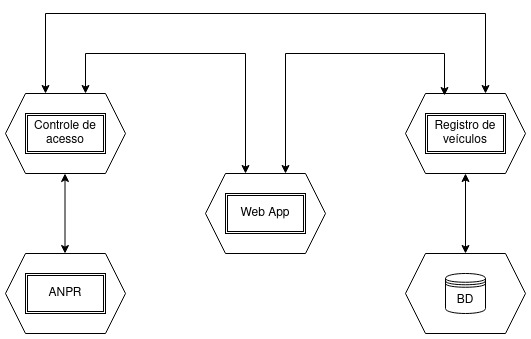
\includegraphics[width=.8\textwidth]{anpr-auth.jpg}
	\caption{Esquema da organização e relacionamento entre os contêineres do sistema}
	\label{fig:anpr-auth}
\end{figure}

A seguir, será apresentada com detalhes a forma com que cada um dos módulos foi desenvolvida e como eles se interagem.

\subsection{Composição de contêineres}

Todos os módulos do sistema são construídos com contêineres Docker, constituindo assim uma aplicação multi-contêiner, a partir de alguma imagem\footnote{Uma "imagem docker" pode ser entendida como uma base ou um \textit{template} sobre o qual o contêiner será inicializado.} padrão ou de uma imagem personalizada.

Para definir e executar a aplicação com múltiplos contêineres, é utilizada a ferramenta Docker Compose\footnote{Página para a documentação oficial do Docker Compose: \url{https://docs.docker.com/compose/}}. Essa ferramenta tem o objetivo de otimizar o processo de construção e execução de múltiplos contêineres, tanto das etapas de desenvolvimento e testes quanto na implantação para produção.

O uso da ferramenta consiste em 3 passos:

\begin{enumerate}
	\item Definir, no arquivo \textit{Dockerfile}, os recursos necessários de cada um dos contêineres da aplicação, como a imagem docker, dependências, usuários e diretórios, portas de serviços e comandos para execução de aplicações, etc. De forma geral, o \textit{Dockerfile} é um \textit{script} que define \textbf{quais} e \textbf{como} instalar e utilizar as ferramentas e aplicações de um contêiner;
	\item Definir, em um arquivo \textit{.yml}, os serviços necessários e a relação entre os contêineres, como interface de rede, portas de serviços, volumes de disco e dependências entre contêineres;
	\item Executar o comando \texttt{docker-compose up} para inicializar todos os contêineres descritos no arquivo \textit{.yml}
\end{enumerate}

Vale ressaltar que, apesar do controle ser realizado em um único arquivo, em um cenário de atualização, o Docker Compose apenas reconstruirá o contêiner que possuir alguma modificação.

\subsection{ANPR}

O módulo ANPR é o responsável por realizar o processamento das imagens dos veículo e devolver o texto de sua placa. Para tal, foi utilizado a biblioteca de código-aberto OpenALPR\footnote{Endereço do repositório e documentação da biblioteca: \url{https://github.com/openalpr/openalpr}} e foi implementado uma API REST com o \textit{framework} Java Spring-Boot para processar as requisições de leitura de placas.

A Figura~\ref{fig:anpr4j-data} ilustra o fluxo das requisições de leitura de placa para o contêiner de ANPR.

\begin{figure}[ht]
	\centering
	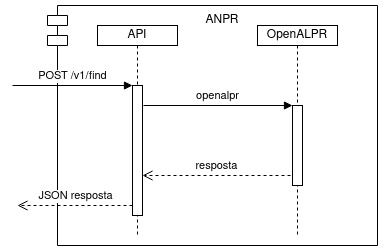
\includegraphics[width=.8\textwidth]{anpr4j-data.jpg}
	\caption{Fluxo de requisições no contêiner de ANPR}
	\label{fig:anpr4j-data}
\end{figure}

A biblioteca OpenALPR, ao receber uma imagem, realiza uma série de passos para detectar ...

\subsection{Banco de Dados (BD)}

Este é o módulo responsável pela persistência dos dados usados pelo sistema, construído com uma imagem do MongoDB\footnote{Página oficial do MongoDB: \url{https://www.mongodb.com/}. Página para a imagem Docker do MongoDB: \url{https://hub.docker.com/_/mongo}}. Ele se encontra em um contêiner próprio para fins de controle de eventuais atualizações e uso de volume de disco, uma vez que a lógica da persistência dos dados se encontra no módulo descrito na sub-seção seguinte.

\subsection{Registro de veículos}


\subsection{Controle de acesso}


\subsection{\textit{Web App}}

O módulo \textit{Web App} 






\section{Resultados} 

\begin{quotation}
	\texttt{\\
		/anpr-auth\\
		+-- /mongo\\
		+-- /alpr4j\\
		|   +-- Dockerfile\\
		|   +-- ...\\
		+-- /check4j\\
		|   +-- Dockerfile\\
		|   +-- ...\\
		+-- /vehiclespy\\
		|   +-- Dockerfile\\
		|   +-- ...\\
		+-- /anpr-ng\\
		|   +-- Dockerfile\\
		|   +-- ...\\
		+-- docker-compose.yml\\}
\end{quotation}

Lorem ipsum dolor sit amet, consectetur adipiscing elit. Etiam at tellus sed diam condimentum tempus. Morbi sagittis ante ex, sed molestie mi euismod sed. Lorem ipsum dolor sit amet, consectetur adipiscing elit. In in elementum dui. Aliquam eget cursus erat. Quisque porttitor vitae metus pulvinar commodo. Vivamus vel ipsum quis diam cursus vulputate vitae at metus. Morbi at quam in mauris lobortis varius. Etiam venenatis lacinia felis quis viverra. Quisque volutpat ac nisl ut gravida. Etiam auctor lacus a nisi fermentum blandit. Fusce at luctus elit, at fringilla est. Nunc nunc nibh, tempor id imperdiet nec, porttitor non tortor.

Sed eros augue, pharetra at dignissim sed, dignissim in odio. Praesent id maximus tellus. Fusce nec condimentum arcu, efficitur sollicitudin dolor. Suspendisse molestie iaculis diam ut tincidunt. Sed ultricies massa sit amet ex convallis, at porttitor nulla eleifend. In ut varius ipsum. Aliquam molestie vestibulum purus, eu rhoncus nisl commodo sit amet. Donec ac ex nisl. Nullam ultrices lectus ipsum, non porta nunc vehicula id. 

\section{Conclusão}

Lorem ipsum dolor sit amet, consectetur adipiscing elit. Etiam at tellus sed diam condimentum tempus. Morbi sagittis ante ex, sed molestie mi euismod sed. Lorem ipsum dolor sit amet, consectetur adipiscing elit. In in elementum dui. Aliquam eget cursus erat. Quisque porttitor vitae metus pulvinar commodo. Vivamus vel ipsum quis diam cursus vulputate vitae at metus. Morbi at quam in mauris lobortis varius. Etiam venenatis lacinia felis quis viverra. Quisque volutpat ac nisl ut gravida. Etiam auctor lacus a nisi fermentum blandit. Fusce at luctus elit, at fringilla est. Nunc nunc nibh, tempor id imperdiet nec, porttitor non tortor.

\textit{trabalhos futuros}

\bibliographystyle{sbc}
\bibliography{sbc-template}

\end{document}
